\chapter{Analysis and prediction of seiyuu popularity}

Popularity is an abstract criterion that must be defined as a numerical metric in order to be used for analysis and prediction. Since we are using MAL database and it has a social component, seems logic to use member\_favorites as a representation of popularity. We can also get popularity and score of anime from opinions of the same set of users.\\

In terms of distribution \textit{popularity} is highly unequal \---as we can observe in Fig.~\ref{fig:popularityDistribution}\--- having a lot of seiyuu which are no member favorites and only a few who are favorite of more than 10000 members. It's good to keep in mind that users can favorite multiple seiyuu.

\begin{figure}[!h]
	\begin{center}
	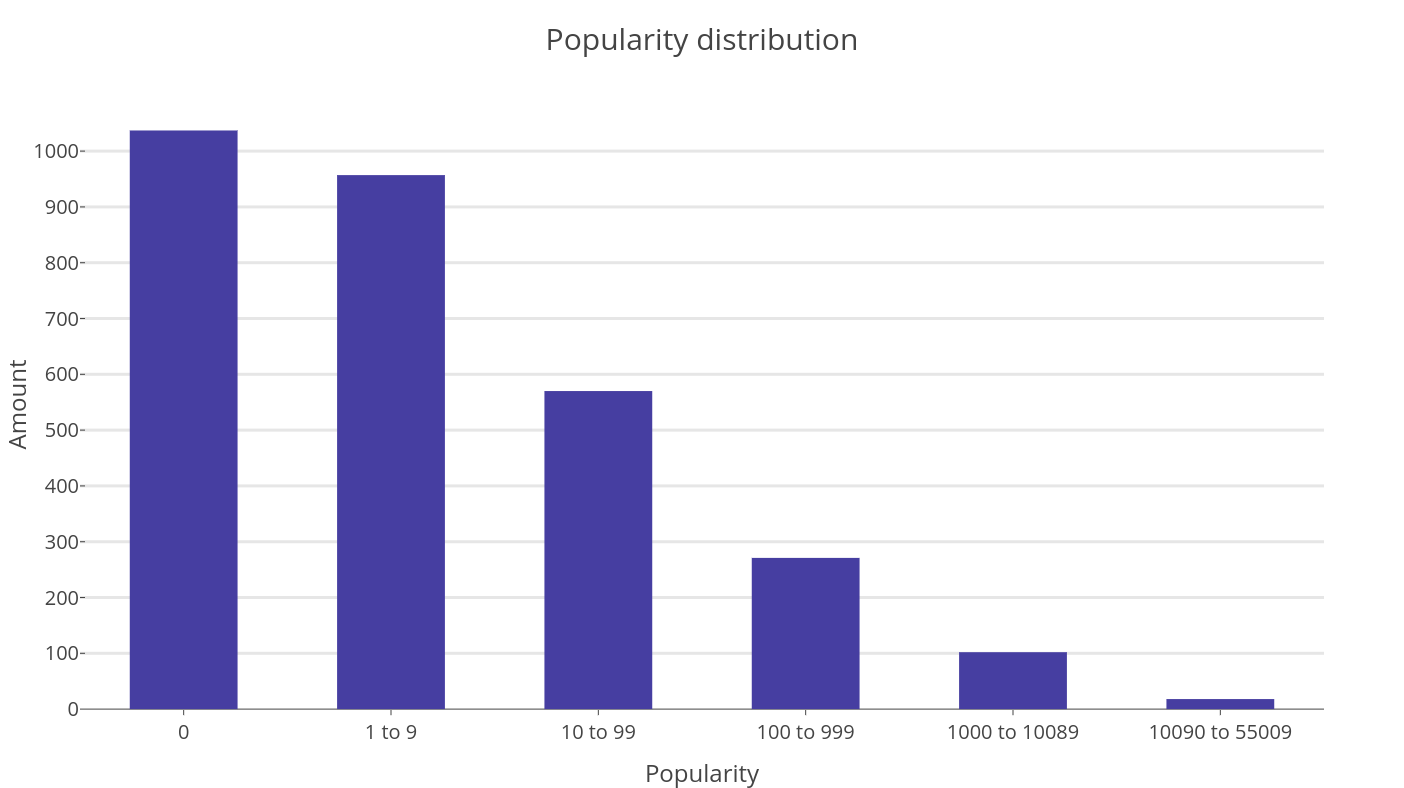
\includegraphics[width=\columnwidth]{graphics/popularityDistribution.png}
	\caption{Amount of seiyuu with that popularity, divided into groups for better visualization.}
	\label{fig:popularityDistribution}
	\end{center}
\end{figure}

\newpage

Some metrics about popularity:
\begin{itemize}
	\item Mean:    289.55
	\item Median:    2.0
	\item Max:    55018
	\item Min:    0 
	\item 1037 values equal to zero
	\item Only 120 values bigger than 1000
\end{itemize}

\begin{table}[!h]
	\begin{center}
	\caption{Top 10 popular seiyuu}
	\label{tab:top10Popularity}
	\begin{tabular}{|l|c|l|}
		\hline
		Name & Popularity & Some popular roles of them\\ 
		\hline
		Kana Hanazawa & 56637 & \textit{Angel Beats!}: Tachibana, Kanade \\ 
		 & & \textit{Steins;Gate}: Shiina, Mayuri \\ 
		 & & \textit{Psycho-Pass}: Tsunemori, Akane \\
		\hline
		Hiroshi Kamiya & 49685 & \textit{Shingeki no Kyojin}: Levi, \\ 
		 & & \textit{Noragami}: Yato \\ 
		 & & \textit{Durarara!!}: Orihara, Izaya \\ 
		\hline
		Mamoru Miyano & 43942 & \textit{Death Note}: Yagami, Light \\ 
		 & & \textit{Steins;Gate}: Okabe, Rintarou \\ 
		 & & \textit{Soul Eater}: Death the Kid \\ 
		\hline
		Rie Kugimiya & 31668 & \textit{Toradora!}: Aisaka, Taiga \\ 
		 & & \textit{Fairy Tail}: Happy \\ 
		 & & \textit{Fullmetal Alchemist}: Elric, Alphonse \\
		\hline
		Jun Fukuyama & 26811 & \textit{Code Geass: Hangyaku no Lelouch}: Lamperouge, Lelouch, \\ 
		 & & \textit{Ao no Exorcist}: Okumura, Yukio \\ 
		 & & \textit{Noragami}: Kazuma \\ 
		\hline
		Miyuki Sawashiro & 26501 & \textit{Sword Art Online II}: Asada, Shino \\ 
		 & & \textit{Durarara!!}: Sturluson, Celty \\ 
		 & & \textit{Highschool of the Dead}: Busujima, Saeko \\
		\hline
		Tomokazu Sugita & 24449 & \textit{Suzumiya Haruhi no Yuuutsu}: Kyon \\
		 & & \textit{JoJo no Kimyou na Bouken (TV)}: Joestar, Joseph \\ 
		 & & \textit{Gintama}: Sakata, Gintoki \\
		\hline
		Daisuke Ono & 24080 & \textit{Durarara!!}: Heiwajima, Shizuo \\ 
		 & & \textit{Kuroshitsuji}: Michaelis, Sebastian \\ 
		 & & \textit{Suzumiya Haruhi no Yuuutsu}: Koizumi, Itsuki \\ 
		\hline
		Saori Hayami & 18322 & \textit{Koe no Katachi}: Nishimiya, Shouko \\ 
		 & & \textit{Owari no Seraph}: Hiiragi, Shinoa \\ 
		 & & \textit{Mahouka Koukou no Rettousei}: Shiba, Miyuki \\
		\hline
		Aya Hirano & 18094 & \textit{Fairy Tail}: Heartfilia, Lucy \\ 
		 & & \textit{Kiseijuu: Sei no Kakuritsu}: Migi \\ 
		 & & \textit{Suzumiya Haruhi no Yuuutsu}: Suzumiya, Haruhi \\
		\hline
	\end{tabular}
	\end{center}
\end{table}

\newpage
\section{Correlation with only one feature}
Our first approach to explaining popularity was using Pearson correlation.

\begin{figure}[!h]
	\begin{flushleft}
	\makebox[\textwidth][c]{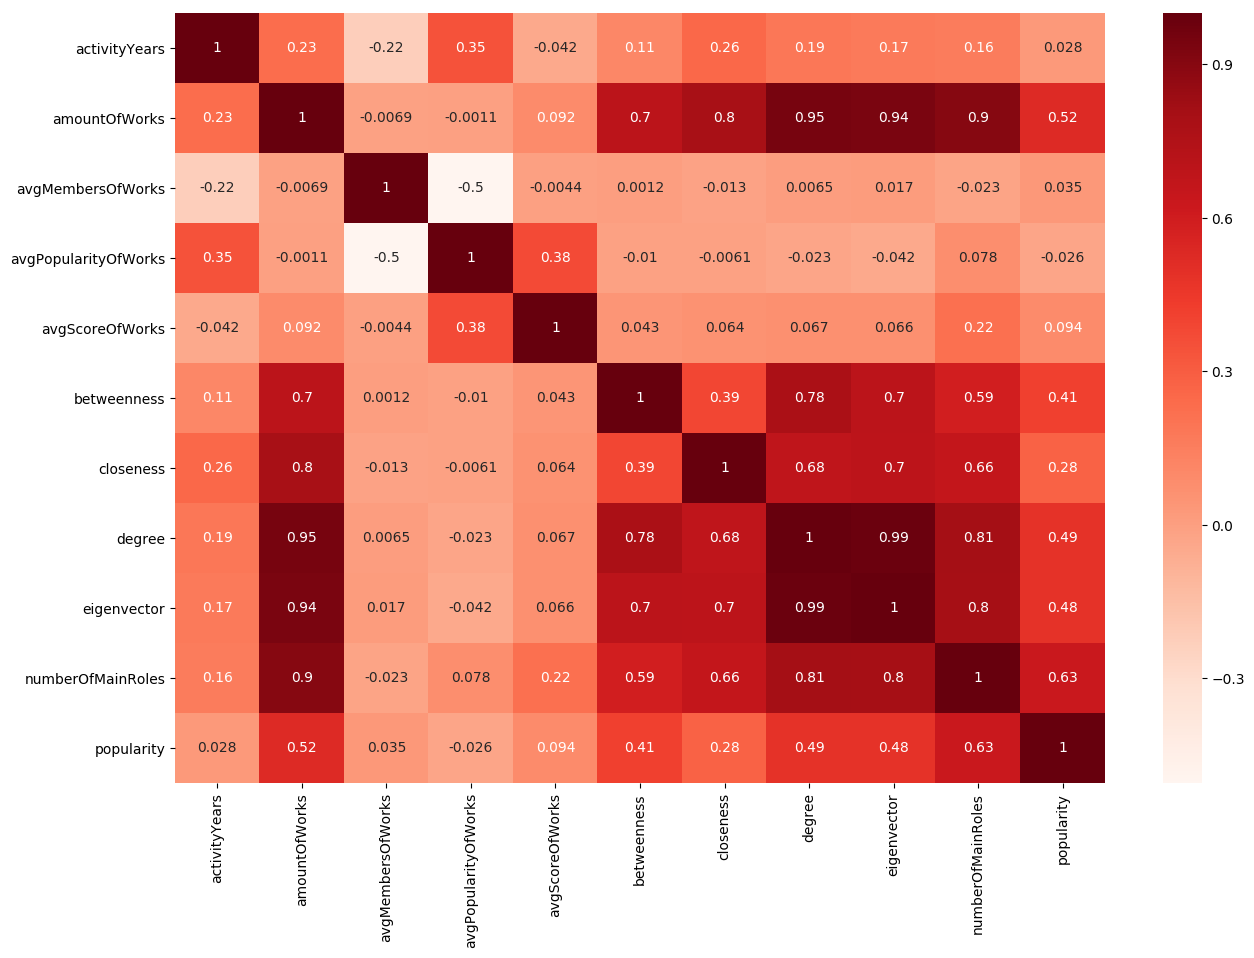
\includegraphics[width=1.7\columnwidth]{graphics/10Works_correlation_Pearson_allWorks.png}}%
	\caption{Pearson correlation between popularity and attribute of nodes (using all works).}
	\label{fig:pearsonCorrAllWorks}
	\end{flushleft}
\end{figure}

As shown on Fig.~\ref{fig:pearsonCorrAllWorks} a fairly big correlation can be seen between popularity and amount of works. This attribute doesn't have the biggest correlation with popularity but "number of main roles" was added to the end of this investigation since we didn't had the data for doing so before. Number of main roles and amount of works have a strong correlation with each other (0.9) but they have different influence over popularity, this means they provide distinct information.

We are showing only average of values for work's attributes (ex. favorites) mostly for better visualization but for predictions we use sum, mean, median and maximum.

Since our dataset is biased in favor of more modern anime we thought of correlate with more recent works only. But, how recent? Last 5, 10 or 20 years? Thus correlation between popularity and works from different data frames was analyzed, Fig.~\ref{fig:correlationPopRecentWorks}.

\begin{figure}[!h]
	\begin{center}
	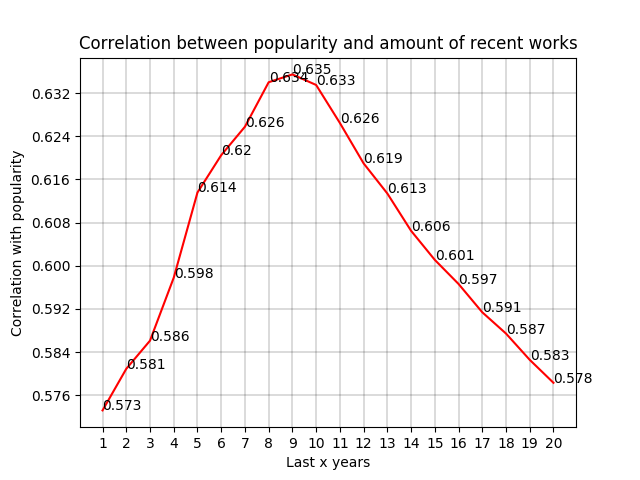
\includegraphics[width=\columnwidth]{graphics/correlationPopRecentWorks.png}
	\caption{Last \textit{X} years means works from 2018-\textit{X} to present.}
	\label{fig:correlationPopRecentWorks}
	\end{center}
\end{figure}

The best result was given by recent works from last 9 years. Therefore, this definition of recent works was used from there on.

Fig.~\ref{fig:pearsonCorrRecentWorks} shows the result of running Pearson again but using information from last 9 years of works only. It's important to clarify that we didn't build the network using only last 9 years, so betweenness centrality and degree are exactly the same as before. We left "amount of works" attribute for easy comparision against "amount of recent works".

\begin{figure}[!h]
	\begin{flushleft}
	\makebox[\textwidth][c]{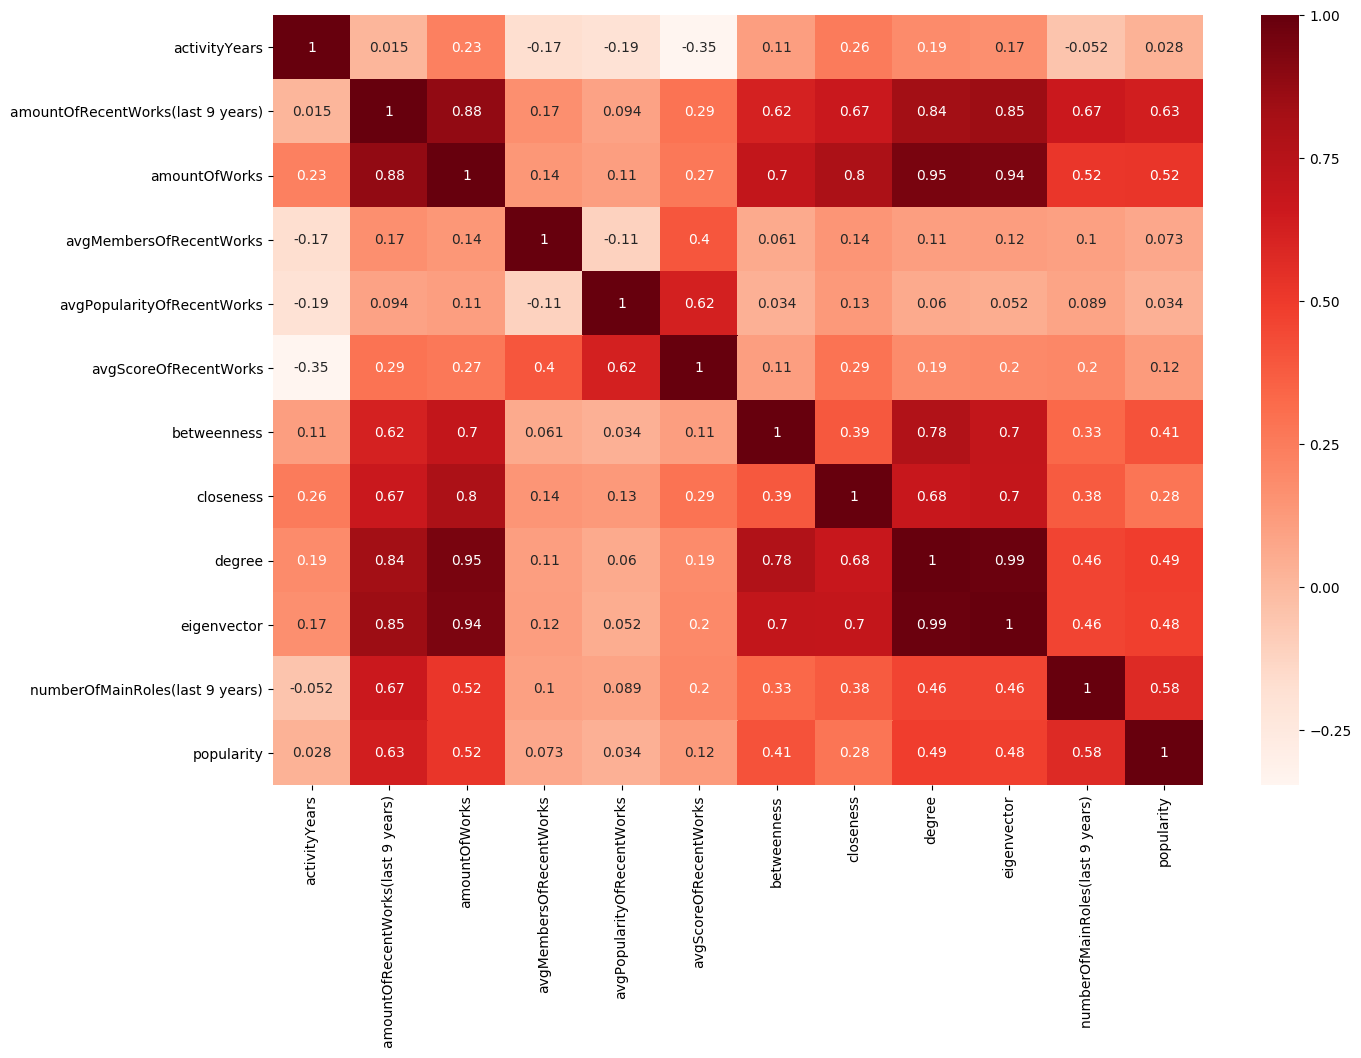
\includegraphics[width=1.7\columnwidth]{graphics/10Works_correlation_Pearson_recentWorks.png}}%
	\caption{Pearson correlation between popularity and attribute of nodes (using recent works only).}
	\label{fig:pearsonCorrRecentWorks}
	\end{flushleft}
\end{figure}

\FloatBarrier
\subsection{Why last 9 years of works has more correlation?}
Graphics of some characteristics of works divided by years were made, trying to shed some light over why works from last 9 years were more "important".

\begin{sidewaysfigure}
	\centering
	\begin{subfigure}{.55\columnwidth}
		\centering
		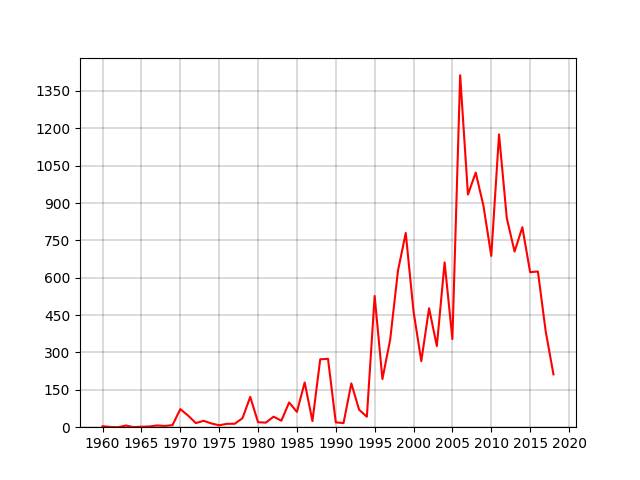
\includegraphics[width=\columnwidth]{graphics/avgFavorites.png}
		\caption{Average amount of favorites per year.}
		\label{fig:avgFavorites}
	\end{subfigure}%
	\begin{subfigure}{.55\columnwidth}
		\centering
		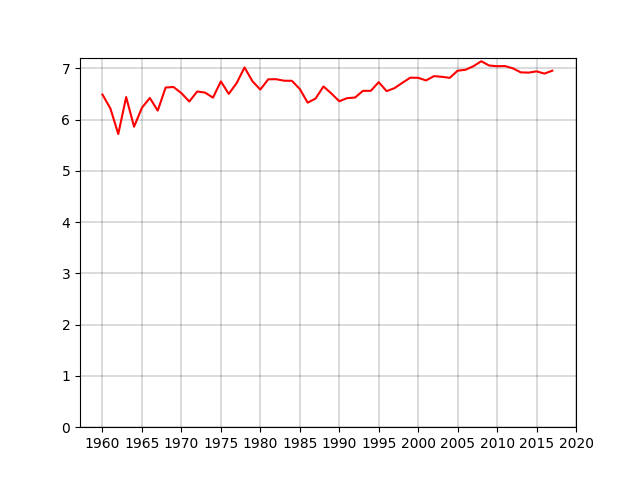
\includegraphics[width=\columnwidth]{graphics/avgScores.png}
		\caption{Average score per year.}
		\label{fig:avgScores}
	\end{subfigure}
	\begin{subfigure}{.55\columnwidth}
		\centering
		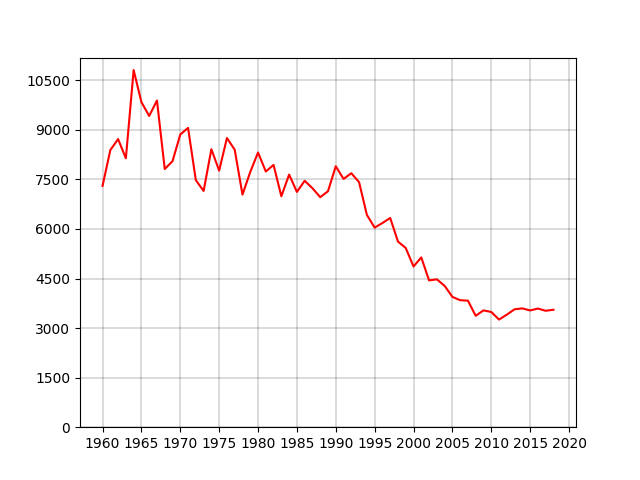
\includegraphics[width=\columnwidth]{graphics/avgPopularities.png}
		\caption{Average popularity per year.}
		\label{fig:avgPopularities}
	\end{subfigure}%
	\begin{subfigure}{.55\columnwidth}
		\centering
		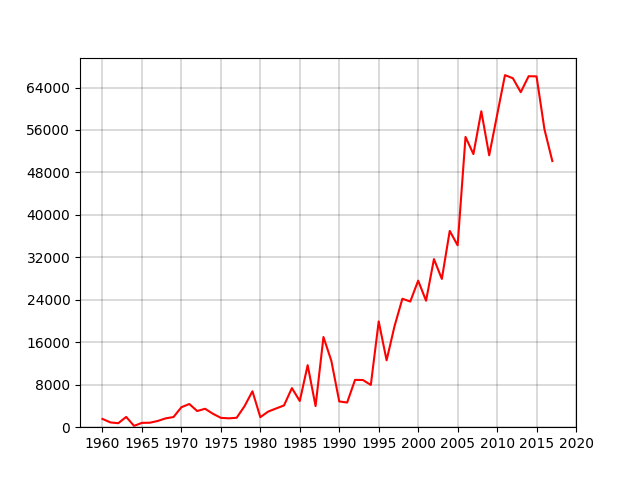
\includegraphics[width=\columnwidth]{graphics/avgMembers.png}
		\caption{Average amount of members per year.}
		\label{fig:avgMembers}
	\end{subfigure}
	\caption{Averages of some atributes of anime divide by year.}
	\label{fig:averages}
\end{sidewaysfigure}

Fig.~\ref{fig:avgFavorites} and ~\ref{fig:avgScores} shows an improvement in average of scores and favorites. 
Biggest peak of favorites is on 2005, this may have to do with the start of MAL (2006), see Fig.~\ref{fig:avgFavorites}. We suppose as users started to use MAL they favorite anime they liked from that year and only some of the old ones; from then on they used the website often and favorite new works as they began airing.

Year 2018 was left out of Fig.~\ref{fig:avgScores} because, since 2018 is not finished yet, the average of scores was unusually small.

As Fig.~\ref{fig:avgPopularities} shows, popularity goes down in last years. But we need to consider that this metrics are from MAL and it could mean, for example, the parameter is in disuse; instead of representing how people feel about new anime.\\

We suppose the attribute "members" of an anime is taken from how many users have it on any of their lists. If that is correct Fig.~\ref{fig:avgMembers} tells us feature of adding anime in watched / watching / plan to watch lists is really used. As for our experience on the web and social media we can confirm this is the most used feature of MAL. So this makes it one of the best metrics to measure "public" as another sense of popularity of anime.\\

As we can see on Fig.~\ref{fig:amountOfWorksPerYear} anime industry is growing bigger each year, of course this is biased by the fact MAL will sure have every adaptation of last year but maybe not for anime from 1980.

\begin{figure}[!h]
	\begin{center}
	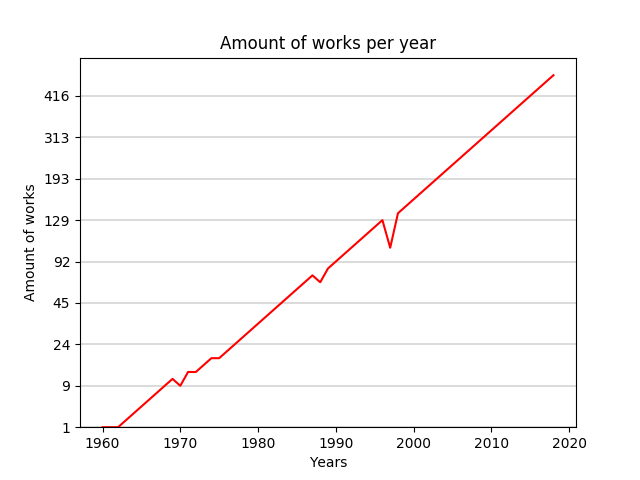
\includegraphics[width=\columnwidth]{graphics/worksPerYear_1960-2018.png}
	\caption{Amount of works divided by years which were aired for the first time.}
	\label{fig:amountOfWorksPerYear}
	\end{center}
\end{figure}

The majority of works are from 1990 to 2018 and half of them are distributed over the last 14 years (2014 to 2018) but as far as we can tell there isn’t anything particular over the last 9 years nor on year 2009. Judging by amount of favorites per year it appears that users have been more active in recent years so this could be one of the reasons.

\section{Correlation with multiple features}
For this section Scikit-learn, a free software machine learning Python library, was used. The node attributes were divided into categories, leaving four distinct types:

\begin{itemize}
	\item Personal data:
	\begin{itemize}
		\item Debut
		\item Gender
		\item Activity years (2018-debut)
	\end{itemize}
	\item Works data:
	\begin{itemize}
		\item Amount
		\item Top 5 genre
		\item Favorites
		\item Score
		\item Popularity
		\item Members
		\item Number of main roles
	\end{itemize}
	\item Recent works data:
	\begin{itemize}
		\item Same as works but for only last 9 years
	\end{itemize}	
	\item Graph data:
	\begin{itemize}
		\item Degree
		\item Betweenness centrality
		\item Closeness
	\end{itemize}
\end{itemize}

Fitting and prediction experiments were run for each category, each combination of 2, 3 and all of them together; using 80\% of seiyuu as train data and the rest as test. This was done for all following models:
\begin{itemize}
	\item DecisionTreeRegressor
	\item DecisionTreeClassifier
	\item LinearRegression
	\item KNeighborsClassifier
	\item LinearDiscriminantAnalysis
	\item GaussianNB
	\item SVM
\end{itemize}

We used r2\_score\footnote{\url{http://scikit-learn.org/stable/modules/model_evaluation.html#r2-score-the-coefficient-of-determination}} for accuracy comparation. Problem is, since popularity variance is really high, we observed some good results in terms of r2\_score values but particular predictions were aloof. 

If we predict without error a seiyuu whose popularity is \textgreater50000 but we make "small" mistakes predicting seiyuu with \textless100 popularity then, is it a good prediction? and having into account more than $\frac{3}{4}$ of them have \textless100 popularity? 

This was happening to our predictions. Since they were on spot for higher popularity values their prediction performance's metrics were good; but in fact they failed on small values, which is the big majority of them. 

Fig.~\ref{fig:scatterPlot_DTC_WR} and Fig.~\ref{fig:scatterPlot_LR_WR} shows some examples.\\

\begin{figure}
	\centering
	\begin{subfigure}{.5\columnwidth}
		\centering
		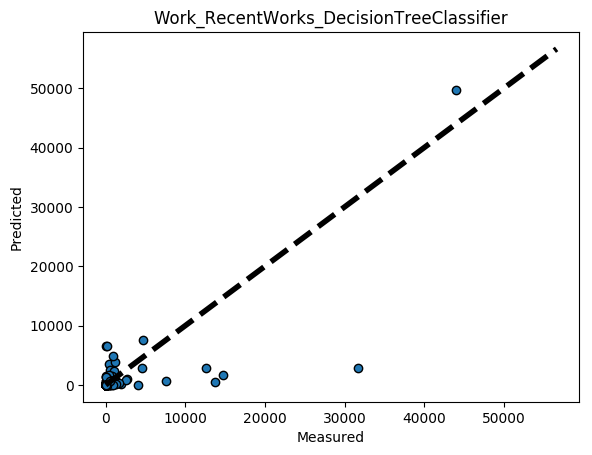
\includegraphics[width=\columnwidth]{graphics/Work_RecentWorks_DecisionTreeClassifier.png}
		\caption{All values.}
	\end{subfigure}%
	\begin{subfigure}{.5\columnwidth}
		\centering
		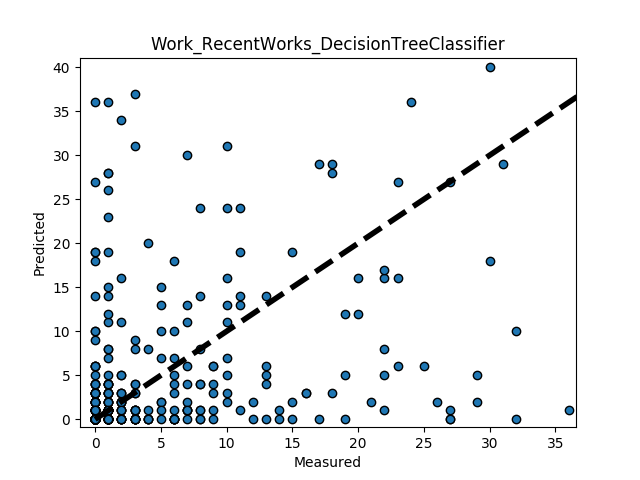
\includegraphics[width=\columnwidth]{graphics/Work_RecentWorks_DecisionTreeClassifierZOOM.png}
		\caption{If we zoom in we can tell it's actually bad predictions.}
	\end{subfigure}
	\caption{Scatter plot showing predicted / measured for Decision Tree Classifier using model Work + RecentWorks.}
	\label{fig:scatterPlot_DTC_WR}
\end{figure}

\begin{figure}
	\centering
	\begin{subfigure}{.5\columnwidth}
		\centering
		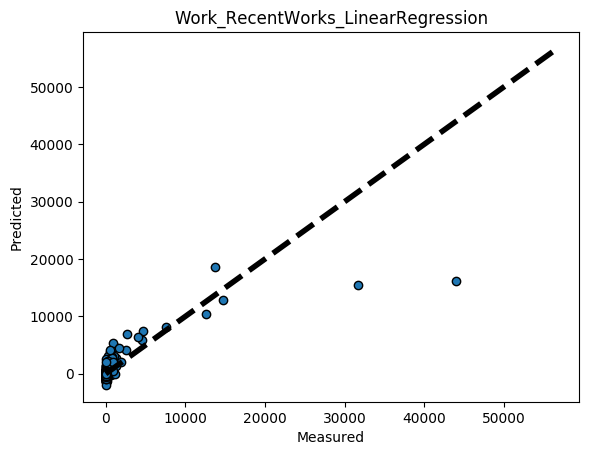
\includegraphics[width=\columnwidth]{graphics/Work_RecentWorks_LinearRegression.png}
		\caption{All values.}
		\label{fig:avgFavorites}
	\end{subfigure}%
	\begin{subfigure}{.5\columnwidth}
		\centering
		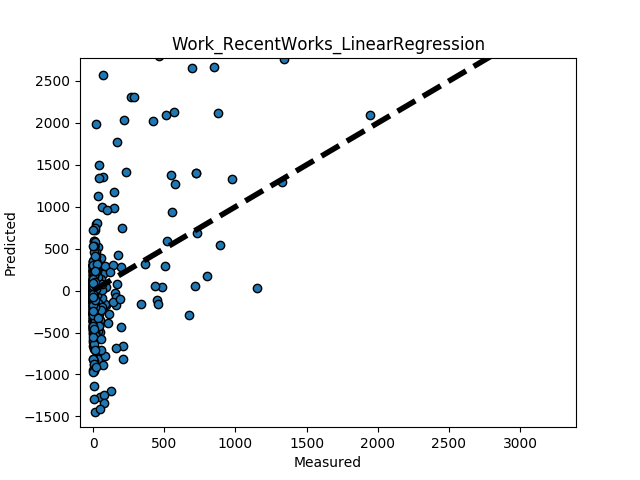
\includegraphics[width=\columnwidth]{graphics/Work_RecentWorks_LinearRegressionZOOM.png}
		\caption{Zoomed in.}
		\label{fig:avgScores}
	\end{subfigure}
	\caption{Scatter plot showing predicted / measured for Linear Regression using model Work + RecentWorks.}
	\label{fig:scatterPlot_LR_WR}
\end{figure}

On the next subchapters we present r2\_score values for each algorithm and each combination of categories. Along with information about which feature is more important, from the Decision Tree Classifier's point of view (for only some of the models).

%-------------------------------------------------------------------------------
\FloatBarrier
\subsection{Only one category}
\begin{table}[!hbt]
	\begin{center}
	\caption{Only one category R2 score results}
	\label{tab:oneCategory}
	\begin{tabular}{lrrrr}
\toprule
{} &  Personal &  Graph &  Work &  RecentWorks \\
\midrule
DecisionTreeClassifier     &     -0.02 &  -3.26 & -2.12 &        -0.59 \\
DecisionTreeRegressor      &     -0.03 &  -1.05 & -0.96 &         0.35 \\
GaussianNB                 &     -0.47 &  -0.57 &  0.01 &         0.03 \\
KNeighborsClassifier       &     -0.02 &   0.04 &  0.07 &         0.10 \\
LinearDiscriminantAnalysis &     -0.02 &  -4.34 &  0.31 &         0.49 \\
LinearRegression           &     -0.00 &   0.13 &  0.31 &         0.48 \\
SVM                        &     -0.02 &  -0.23 & -0.02 &         0.02 \\
\bottomrule
\end{tabular}

	\end{center}
\end{table}

Table.~\ref{tab:oneCategory} reveals that Recent Works is the most performant if we are only using one category.

\begin{figure}[!hbt]
	\centering
	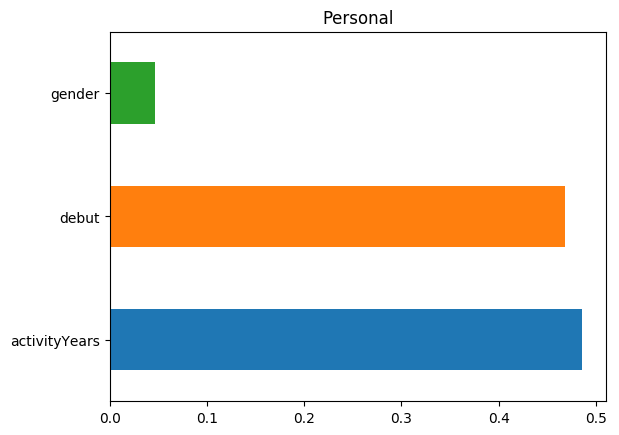
\includegraphics[width=\columnwidth]{graphics/Personal_DTC_featureImportances.png}
	\caption{Feature information contribution for Personal data.}
	\label{fig:DTC_P}
\end{figure}

Fig.~\ref{fig:DTC_P} shows that Decision Tree Classifier firstly uses activity years and debut to distinguish between most clases.

\begin{figure}[!hbt]
	\centering
	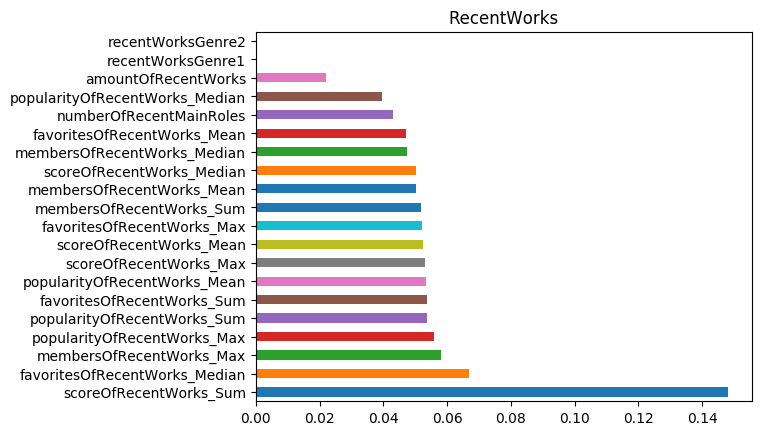
\includegraphics[width=\columnwidth]{graphics/RecentWorks_DTC_featureImportances.png}
	\caption{Feature information contribution for Recent works.}
	\label{fig:DTC_R}
\end{figure}

Decision Tree Classifier has bad performance when using only Recent works data but there's something very interesting about Fig.~\ref{fig:DTC_R}, when using Work and Recent works "number of \textit{recent} main roles" is not used to classify but here it is used; we suppose is because it doesn't provide new information against "number of mail roles" (see Fig.~\ref{fig:DTC_WR}).

%-------------------------------------------------------------------------------
\FloatBarrier
\subsection{Groups of two categories}
\begin{table}[!hbt]
	\begin{center}
	\caption{Two categories R2 score results (R: recent works, P: personal, G: graph, W: work)}
	\label{tab:twoCategories}
	\begin{tabular}{lrrrrrr}
\toprule
{} &   P+G &   P+W &   P+R &   G+W &   G+R &   W+R \\
\midrule
DecisionTreeClassifier     &  0.11 & -0.43 & -1.86 & -0.70 & -2.51 &  0.57 \\
DecisionTreeRegressor      & -2.56 & -1.15 & -0.37 & -0.21 & -0.86 &  0.39 \\
GaussianNB                 & -0.06 &  0.03 &  0.01 &  0.01 &  0.07 &  0.00 \\
KNeighborsClassifier       &  0.10 &  0.15 &  0.03 &  0.08 &  0.25 &  0.08 \\
LinearDiscriminantAnalysis & -0.35 &  0.43 & -0.08 &  0.21 &  0.40 &  0.62 \\
LinearRegression           &  0.38 &  0.57 &  0.38 &  0.52 &  0.33 &  0.63 \\
SVM                        & -0.02 &  0.00 & -0.04 & -0.00 &  0.03 & -0.02 \\
\bottomrule
\end{tabular}

	\end{center}
\end{table}

Table.~\ref{tab:twoCategories} shows ones of the best r2\_scores of all predictions. Decision Tree Classifier, Linear Discriminant Analysis and Linear Regression all did well when using Work + Recent Works model.

\begin{figure}[!hbt]
	\centering
	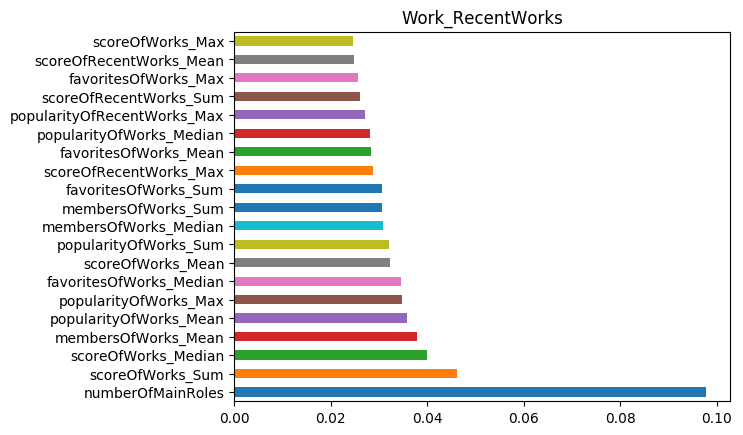
\includegraphics[width=\columnwidth]{graphics/Work_RecentWorks_DTC_featureImportances.png}
	\caption{Feature information contribution for Work + Recent works model.}
	\label{fig:DTC_WR}
\end{figure}

As Fig.~\ref{fig:DTC_WR} reveals number of main roles is a very important feature to classify seiyuu by popularity. We saw earlier that it has a strong correlation.

%-------------------------------------------------------------------------------
\FloatBarrier
\subsection{Groups of three categories}
\begin{table}[!hbt]
	\begin{center}
	\caption{Three categories R2 score results (R: recent works, P: personal, G: graph, W: work)}
	\label{tab:threeCategories}
	\begin{tabular}{lrrrr}
\toprule
{} &  P+G+W &  P+G+R &  P+W+R &  G+W+R \\
\midrule
DecisionTreeClassifier     &  -0.90 &  -8.46 &  -0.72 &  -0.73 \\
DecisionTreeRegressor      &  -1.75 &  -2.12 &  -1.55 &   0.20 \\
GaussianNB                 &   0.01 &   0.05 &   0.04 &   0.02 \\
KNeighborsClassifier       &   0.06 &   0.64 &  -0.04 &   0.18 \\
LinearDiscriminantAnalysis &  -0.16 &  -0.19 &   0.54 &   0.51 \\
LinearRegression           &  -0.96 &  -1.63 &   0.09 &   0.38 \\
SVM                        &  -0.03 &  -0.04 &  -0.03 &  -0.02 \\
\bottomrule
\end{tabular}

	\end{center}
\end{table}

According to Table.~\ref{tab:threeCategories} three categories models have bad performance for most algorithm but it also has the highest (best) value of all. Is achieved by K Neighbors Classifier when using Personal + Graph + Recent works data.

\begin{figure}[!hbt]
	\centering
	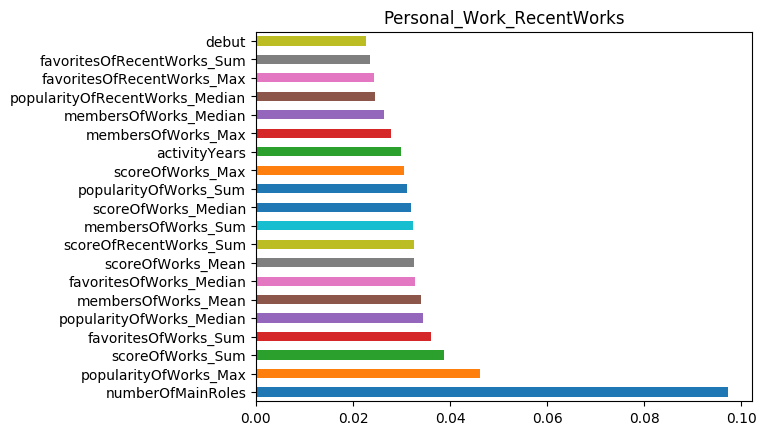
\includegraphics[width=\columnwidth]{graphics/Personal_Work_RecentWorks_DTC_featureImportances.png}
	\caption{Feature information contribution for Personal + Work + Recent works model.}
	\label{fig:DTC_PWR}
\end{figure}

Fig.~\ref{fig:DTC_PWR} tells us, as we already saw before, that number of main roles is a very important feature. Also, notice that number of \textit{recent} main roles does not appear.

%-------------------------------------------------------------------------------
\FloatBarrier
\subsection{All categories}
\begin{table}[!hbt]
	\begin{center}
	\caption{All categories R2 score results}
	\label{tab:allCategories}
	\begin{tabular}{lr}
\toprule
{} &  AllFeatures \\
\midrule
DecisionTreeClassifier     &        -1.51 \\
DecisionTreeRegressor      &         0.04 \\
GaussianNB                 &         0.04 \\
KNeighborsClassifier       &         0.40 \\
LinearDiscriminantAnalysis &         0.53 \\
LinearRegression           &         0.53 \\
SVM                        &         0.01 \\
\bottomrule
\end{tabular}

	\end{center}
\end{table}

Table.~\ref{tab:allCategories} Decision Tree Classifier has bad performance when using all categories, this can be because it overfits train data. Linear Discriminant Analysis and Linear Regression doesn't seem to do that bad, Decision Tree Regressor also. Of course, once we saw the scatter plots particular predictions were wrong most of the times for small values, showing a very different reality from value of metrics.

\begin{figure}[!hbt]
	\centering
	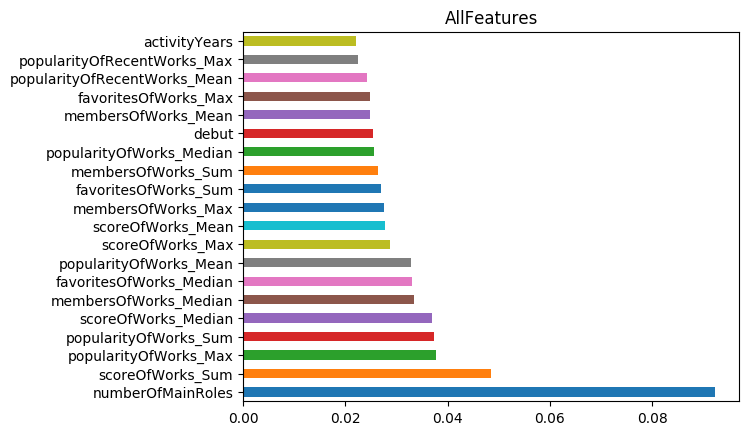
\includegraphics[width=\columnwidth]{graphics/AllFeatures_DTC_featureImportances.png}
	\caption{Feature information contribution for model using all categories.}
	\label{fig:DTC_All}
\end{figure}

As Fig.~\ref{fig:DTC_All} shows, even when using all features "number of main roles" is still the one that separates more values, having almost double importance than the second one (sum of score of works).

%-------------------------------------------------------------------------------
\section{Conclusion}

Since particular predictions were usually wrong (mostly for small values) this couldn't be used in a practical way to predict popularity of new seiyuu nor to recover lost values. 

\textbf{TODO, LO BUENO ES QUE PUDIMOS VER IMPORTANCIA DE LOS FEATURES, QUE NUMBER OF MAIN ROLES ES IMPORTANTE, QUE LAS METRICAS SON DIFICILES DE USAR CUANDO HAY MUCHA VARIANZA?, PUDIMOS COMPARAR LOS DISTINTOS ALGORITMOS, VIENDO CUANDO ERAN MAS O MENOS PERFORMANTES...PO...NE...LE}